\subsection{Strassen's Algorithm Results:}

First test for {\bfseries\itshape Strassen's Algorithm}. The program will plot the {\bfseries\itshape time} that the algorithm takes to make the product of matrices of size {\itshape  n = $2^{4}$}. \hfill \break

{\bfseries\itshape\color{carmine}{Observation:}} {\itshape\color{carmine}{This algorithm has the same complexity always, that is because doesn't has worst or best case.}} \hfill \break

\begin{multicols}{2}
\begin{figure}[H]
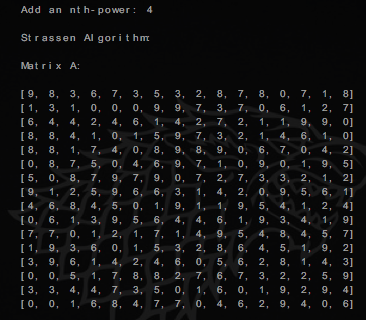
\includegraphics[width = 8cm, height = 5cm]{t1a.png}
\centering \linebreak \linebreak Figure 4.1.0: Matrix A of size n = $2^{4}$.
\end{figure} \hfill 

\begin{figure}[H]
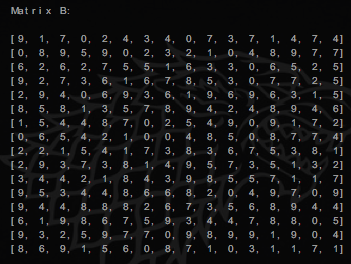
\includegraphics[width = 8cm, height = 5cm]{t1b.png}
\centering \linebreak \linebreak Figure 4.1.1: Matrix B of size n = $2^{4}$.
\end{figure} 
\end{multicols}

\begin{figure}[H]
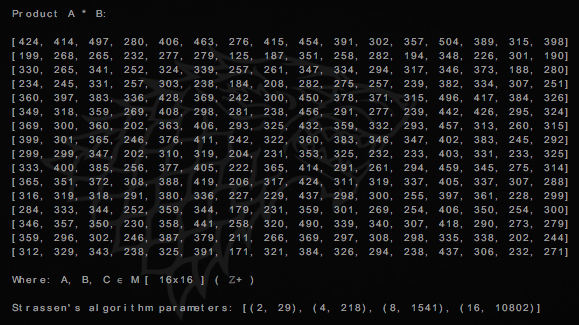
\includegraphics[width = 16.5cm, height = 8cm]{t1c.png}
\centering \linebreak \linebreak Figure 4.1.2: Product of A $\cdot$ B..
\end{figure} 

\pagebreak

\begin{figure}[H]
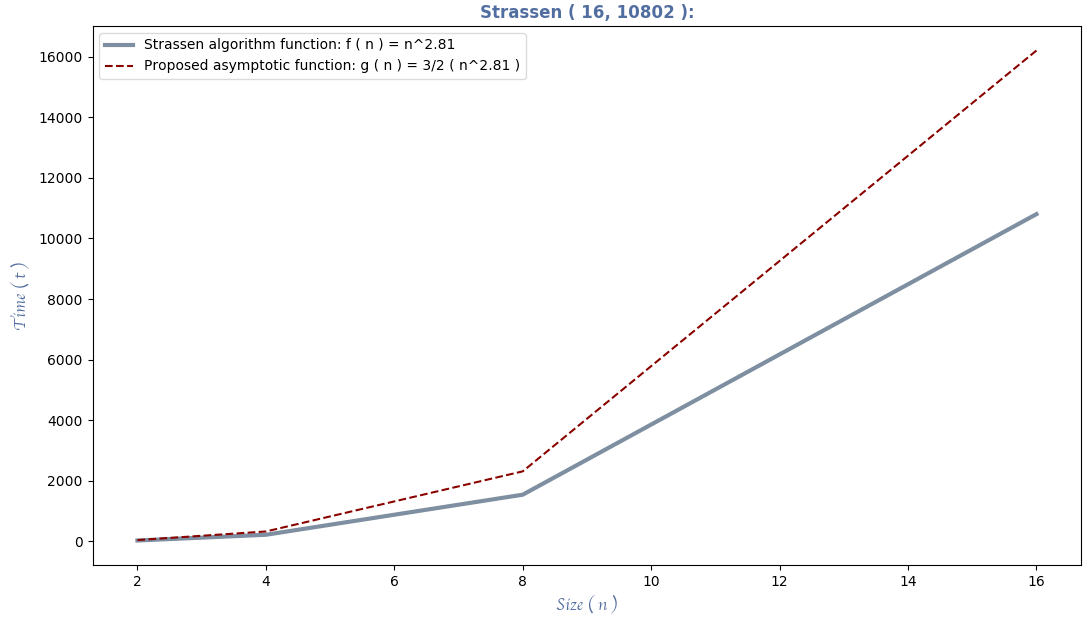
\includegraphics[width = 16.5cm, height = 10cm]{g1.png}
\centering \linebreak \linebreak Figure 4.1.3: Graph for Figure 4.1.2.
\end{figure} \hfill

{\bfseries\itshape\color{carmine}{Observation:}} {\itshape\color{carmine}{The red function it's the proposed one: g ( n ) = $\frac{3}{2}\ \cdot\ n^{2.81}$ and the blue it's the Stranssen's Algorithm complexity: f ( n ) = $n^{2.81}$.}} \hfill \break

\begin{center}
{\Large
\begin{tabular}[.5cm]{ c c c }
\toprule
Size ( $2^{n}$ ) & Time ( t ) \\
\midrule
2 & 29 \\
\cmidrule {1-2}
4 & 218 \\
\cmidrule {1-2}
8 & 1541 \\
\cmidrule {1-2}
16 & 10802 \\
\bottomrule
\linebreak
\end{tabular}}
\linebreak \linebreak Table 1: Plot point for Strassen's Algorithm complexity of Figure 4.1.3.
\end{center}

\pagebreak

Second test for {\bfseries\itshape Strassen's Algorithm}. The program will plot the {\bfseries\itshape time} that the algorithm takes to make the product of matrices of size {\itshape  n = $2^{5}$}. \hfill \break

\begin{multicols}{2}
\begin{figure}[H]
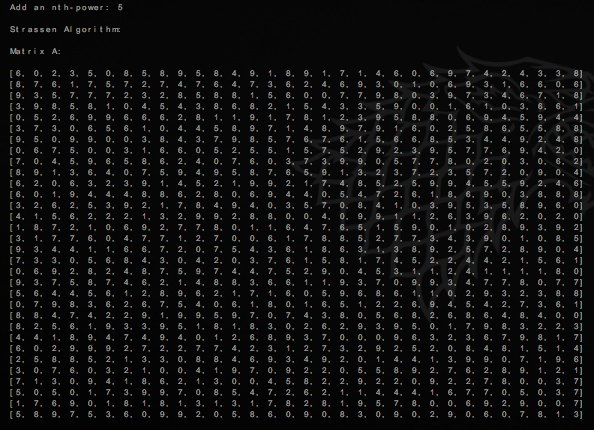
\includegraphics[width = 8cm, height = 5cm]{t2a.png}
\centering \linebreak \linebreak Figure 4.1.4: Matrix A of size n = $2^{5}$.
\end{figure} \hfill 

\begin{figure}[H]
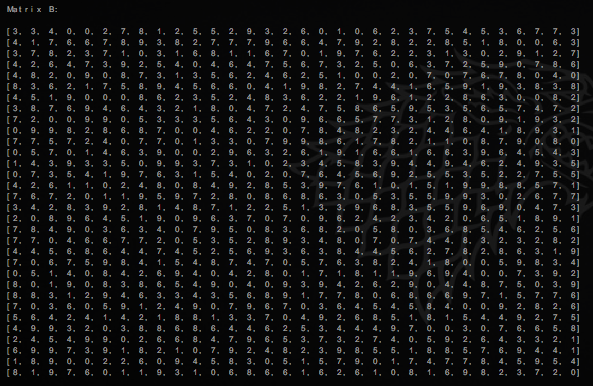
\includegraphics[width = 8cm, height = 5cm]{t2b.png}
\centering \linebreak \linebreak Figure 4.1.5: Matrix B of size n = $2^{5}$.
\end{figure} 
\end{multicols}

\begin{figure}[H]
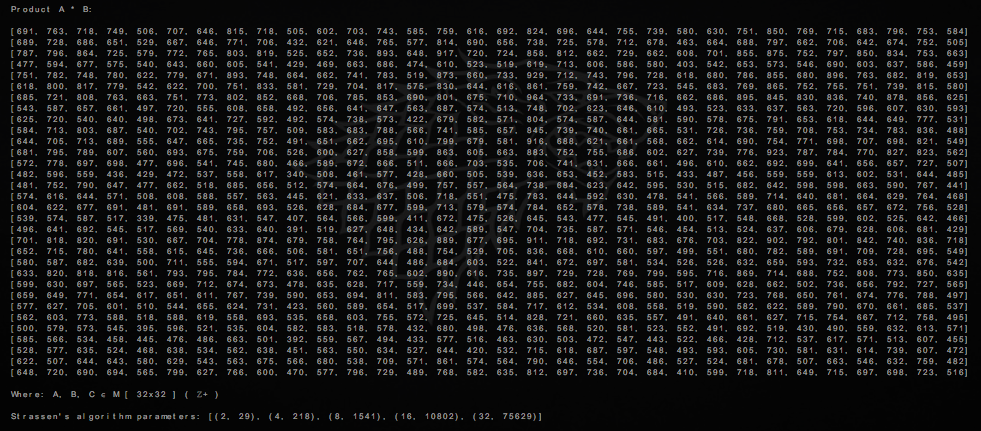
\includegraphics[width = 16.5cm, height = 8cm]{t2c.png}
\centering \linebreak \linebreak Figure 4.1.6: Product of A $\cdot$ B..
\end{figure} 

\pagebreak

\begin{figure}[H]
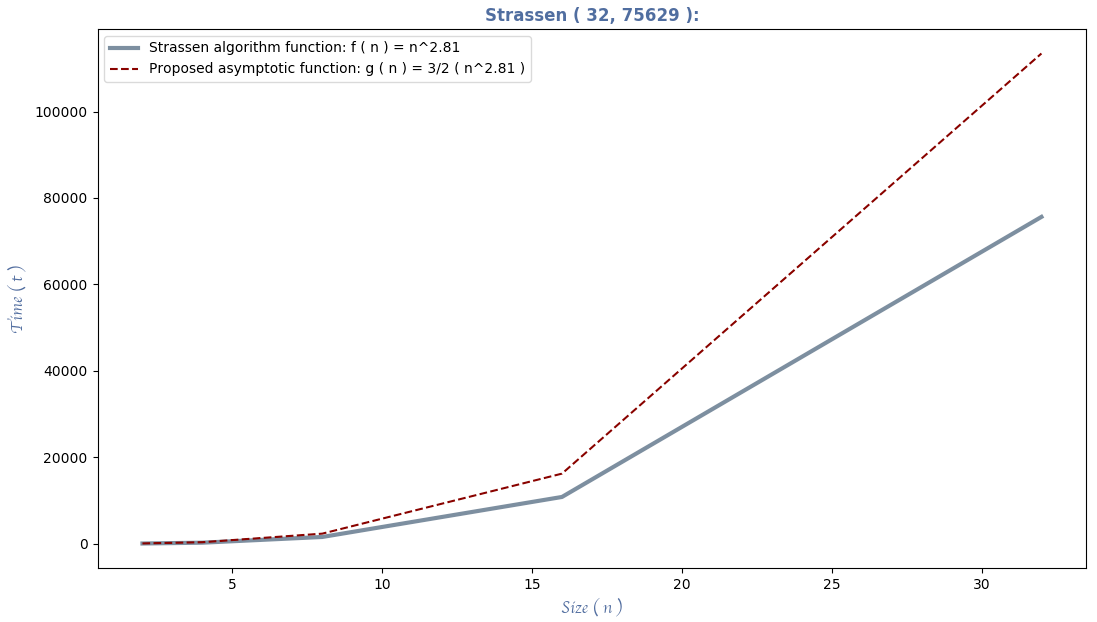
\includegraphics[width = 16.5cm, height = 10cm]{g2.png}
\centering \linebreak \linebreak Figure 4.1.7: Graph for Figure 4.1.6.
\end{figure} \hfill

{\bfseries\itshape\color{carmine}{Observation:}} {\itshape\color{carmine}{The red function it's the proposed one: g ( n ) = $\frac{3}{2}\ \cdot\ n^{2.81}$ and the blue it's the Stranssen's Algorithm complexity: f ( n ) = $n^{2.81}$.}} \hfill \break

\begin{center}
{\Large
\begin{tabular}[.5cm]{ c c c }
\toprule
Size ( $2^{n}$ ) & Time ( t ) \\
\midrule
2 & 29 \\
\cmidrule {1-2}
4 & 218 \\
\cmidrule {1-2}
8 & 1541 \\
\cmidrule {1-2}
16 & 10802 \\
\cmidrule {1-2}
32 & 75629 \\
\bottomrule
\linebreak
\end{tabular}}
\linebreak \linebreak Table 2: Plot point for Strassen's Algorithm complexity of Figure 4.1.7.
\end{center}

\pagebreak